\documentclass[11pt]{article}
\usepackage[french]{babel}

\usepackage[utf8]{inputenc}
\usepackage{palatino}
\usepackage[T1]{fontenc}


\usepackage{url}
\usepackage{amsmath}

\usepackage[top=2cm,bottom=2cm,left=2.1cm,right=2.1cm,headsep=10pt,a4paper]{geometry}
\usepackage{fancyhdr}


\usepackage{graphicx,float} % figure et placement de figure
\usepackage{listings} %%inclusion de programmes

\lstset{
language=C++,
basicstyle=\ttfamily\small, %
identifierstyle=\color{black}, %
keywordstyle=\color{blue}, %
stringstyle=\color{blue}, %
commentstyle=\it\color{green}, %
}

\usepackage{xcolor}

\pagestyle{fancy}
\lhead{}
\chead{\fontsize{10}{10}{M2IM - UCBL - 2014/2015}}
\rhead{}

\lfoot{}
\cfoot{\thepage}
\rfoot{}


\renewcommand{\headrulewidth}{0pt}
\renewcommand{\footrulewidth}{0pt}
%11006689

 \author{\fontsize{14}{14}{Aurélien CHEMIER 10908892 et Romane LHOMME 11006689}}
 \title{\fontsize{16}{16}{{\bf Analyse, aquisition et traitement d’image \\ TP1}}}
 \date{\fontsize{11}{11}{\today}}

\begin{document}

\thispagestyle{empty}
\maketitle

\newpage
\tableofcontents
\newpage

\section{Introduction}

	Dans le cadre de ce projet d’analyse d’image, nous devons implémenter une méthode de détection de contours, à l’aide des filtres vus en cours. 
	Ensuite, une étape de traitement et d'affinage des contours  sera effectuer afin d'avoir un meilleur résultat.
	Ce rapport à pour but de présenter et d'expliquer nos choix lors de ces différentes étapes.

	\section{Technologies utilisées}

	Ce programme de detection de contour a été fait en C++ qui est un langage objet que nous avons l'habitude d'utiliser.

	Pour manipuler les images, nous avons choisi d'utiliser OpenCV, une bibliothèque graphique spécialisée dans le traitement d'image en temps réel.
	Cette librairie a plusieurs avantages :
	\begin{itemize}
		\item Elle est gratuite.
		\item Elle permet une gestion simple des images (lecture, écriture, sauvegarde...).
	\end{itemize}

	L'utilisation de notre programme se fait en ligne de commande.

	Tous nos tests ont été fait sur l'image "Lena", un classique du traitement d'image.

	\begin{figure}[H]
		\centering
		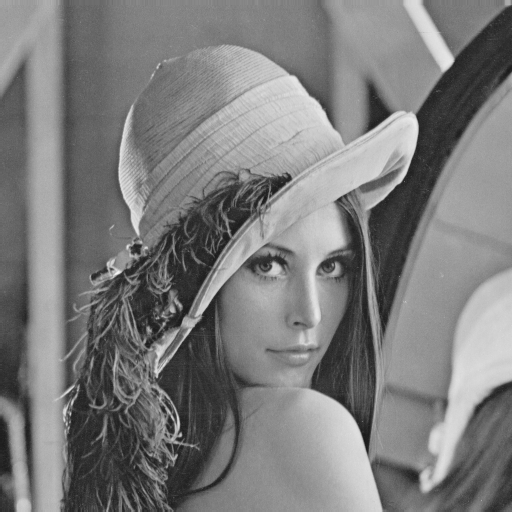
\includegraphics[scale=0.20]{Image/lena.png}
		\caption{Lena}
		\label{fig:Lena}
	\end{figure}

\section{Détection des contours}
	
	L'étape de détection des contours se fait uniquement sur des images en niveaux de gris.

	Dans un premier temps, on procède au calcul du vecteur gradient en chaque point de l'image.
	La méthode demandée consiste à appliquer des opérateurs (ou masques) de convolution (tableau MxM).

	Pour chaque Pixel de l'image, on fait la somme du produit des pixels voisins avec la case du filtre correspndante, comme le montre le code suivant.

	\begin{lstlisting}[caption={filtre.h},language=C++,label=filtreh]
		for (i = 0; i < 3; ++i)
		{
			for (j = 0; j < 3; ++j)
			{ 
				gradient += p[i][j] * Filtre[i][j];	
			}
		}
	\end{lstlisting}
	Le pixel sur lequel s'applique le filtre se situe au milieu de celui ci, ici en position 1,1.

	Le gradient est ensuite normalisé entre 0 et 255 et devient la valeur du pixel courant dans l'image filtrée.

	Tous les filtres appliqués dans ce TPs sont de dimension 3x3.

	\subsection{Implémentation}

		Pour coder ces filtres, nous avons une classe mère filtre.h. 
		\subsubsection{filtre.h}

		\begin{lstlisting}[caption={Classe filtre},language=C++,label=filtre]
		class filtre
		{
		private:
			std::vector<std::vector<int> > GV; //filtre vertical
			std::vector<std::vector<int> > GH; //filtre horizontal
			std::vector<std::vector<int> > Diag; //filtre diagonal

			//utile pour l'affinage des points
			//gradients horizontaux
			std::vector<std::vector<int> > filtreH; 
			//gradients verticaux
			std::vector<std::vector<int> > filtreV; 

			//image modele
			IplImage img;

			//les dimensions de l'image
			unsigned int nbLigne;
			unsigned int nbColonne;
		};
		\end{lstlisting}

		La classe contient également des getters et des setters pour acceder à ses différents éléments.

		Les différents algorithmes de tris sont également dans la classe filtre.

		\subsubsection{Classes filles}

			Les classes filles héritent de filtre.h et permettent d'initialiser les masques horitaux, verticaux et diagonaux avec les valeurs correspondantes au filtre utilisé.

		\subsubsection{Fonction de tri}

			Les différentes fonctions de tri fonctionnent sur le même schéma: 
			\begin{itemize}
			\item La fonction s'applique sur l'image stocké dans le filtre.
			\item Elle retourne une image de même dimension que l'image modèle.
			\end{itemize}


	\subsection{Filtre de base} 

	\begin{itemize}
		\item Prewitt

			\begin{tabular}{cccc}
				horizontal &
				$
				\begin{pmatrix}
					1 & 0 & -1 \\
					1 & 0 & -1 \\
					1 & 0 & -1
				\end{pmatrix}
				$
				&
				vertical &
				$
				\begin{pmatrix}
				1 & 1 & 1 \\
				0 & 0 & 0 \\
				-1 & -1 & -1
				\end{pmatrix}
				$
			\end{tabular}

		\item Sobel

			\begin{tabular}{cccc}
				horizontal &
				$
				\begin{pmatrix}
				1 & 0 & -1 \\
				2 & 0 & -2 \\
				1 & 0 & -1
				\end{pmatrix}
				$
				&
				vertical &
				$
				\begin{pmatrix}
				1 & 2 & 1 \\
				0 & 0 & 0 \\
				-1 & -2 & -1
				\end{pmatrix}
				$
			\end{tabular}

		\item Kisrch

			\begin{tabular}{cccc}
				horizontal &
				$
				\begin{pmatrix}
				-3 & -3 & 5 \\
				-3 & 0 & 5 \\
				-3 & -3 & 5
				\end{pmatrix}
				$
				&
				vertical &
				$
				\begin{pmatrix}
				-3 & -3 & -3 \\
				-3 & 0 & -3 \\
				5 & 5 & 5
				\end{pmatrix}
				$
			\end{tabular}
			
			\item D'autres masques peuvent être utilisés.
	\end{itemize}

	Ces différents filtres appliqués à Lena donnent : 

	\begin{figure}[H]
		\begin{minipage}[c]{.46\linewidth}
			\centering
			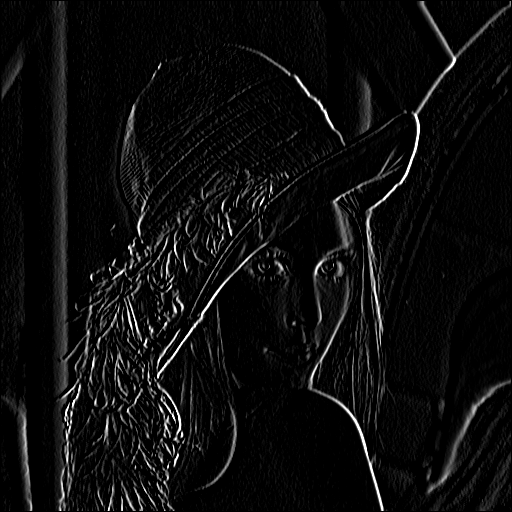
\includegraphics[scale=0.25]{Image/filtrePrewittHorizontal.png}
			\caption{Prewitt Horizontal}
			\label{fig:PrewittHorizontal}
		\end{minipage} \hfill
		\begin{minipage}[c]{.46\linewidth}
		\centering
			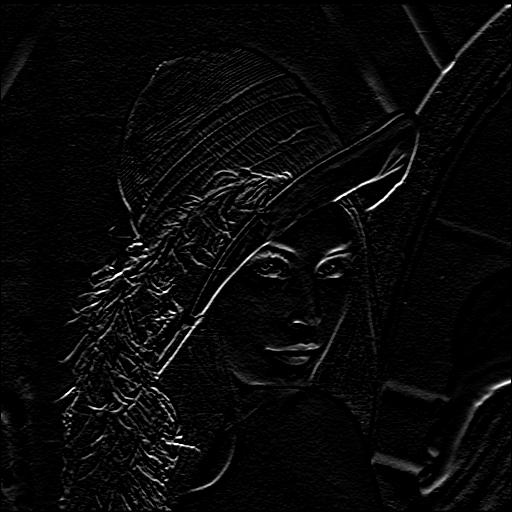
\includegraphics[scale=0.25]{Image/filtrePrewittVertical.png}
			\caption{Prewitt Vertical}
			\label{fig:PrewittVertical}
		\end{minipage}
		\begin{minipage}[c]{.46\linewidth}
			\centering
			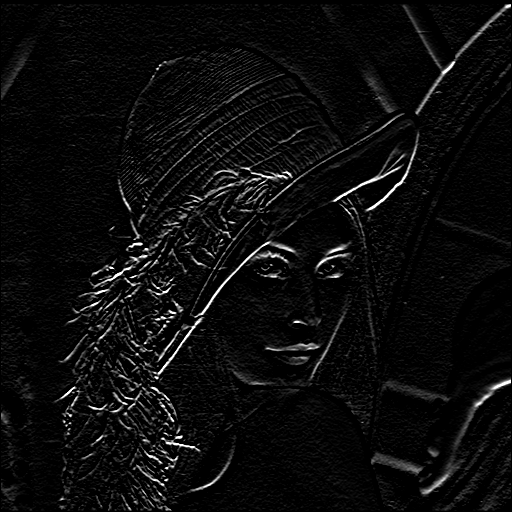
\includegraphics[scale=0.25]{Image/filtreSobelHorizontal.png}
			\caption{Sobel Horizontal}
			\label{fig:SobelHorizontal}
		\end{minipage} \hfill
		\begin{minipage}[c]{.46\linewidth}
		\centering
			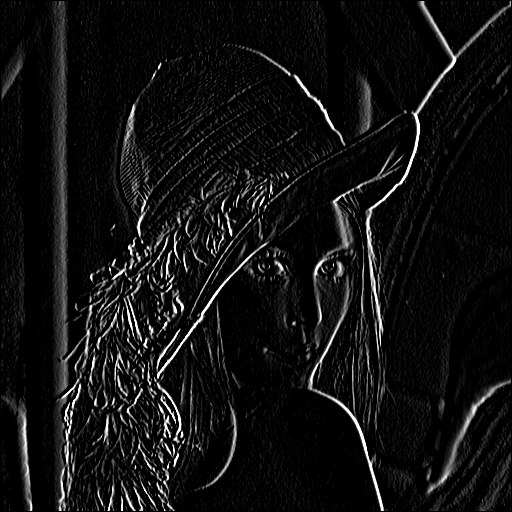
\includegraphics[scale=0.25]{Image/filtreSobelVertical.png}
			\caption{Sobel Vertical}
			\label{fig:SobelVertical}
		\end{minipage}
		\begin{minipage}[c]{.46\linewidth}
			\centering
			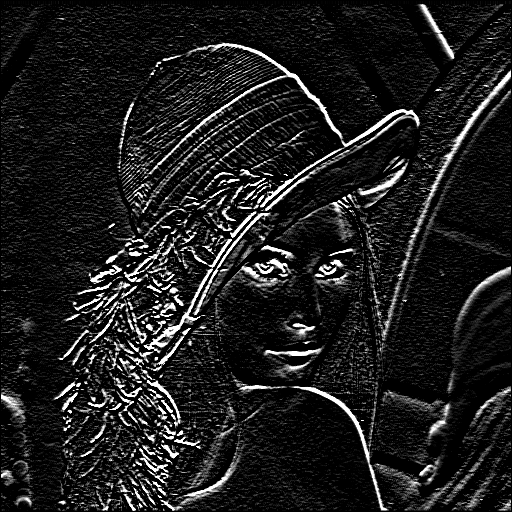
\includegraphics[scale=0.25]{Image/filtreKirschHorizontal.png}
			\caption{Kirsch Horizontal}
			\label{fig:KirschHorizontal}
		\end{minipage} \hfill
		\begin{minipage}[c]{.46\linewidth}
		\centering
			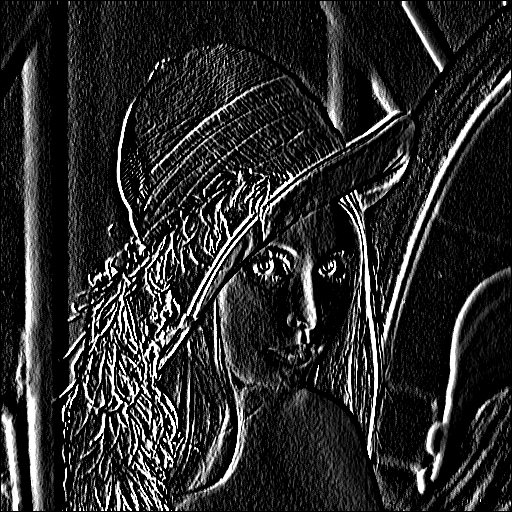
\includegraphics[scale=0.25]{Image/filtreKirschVertical.png}
			\caption{Kirsch Vertical}
			\label{fig:KirschVertical}
		\end{minipage}
	\end{figure}

	La complexité de cette méthode est de l’ordre \[w \times h\] avec:
	\begin{itemize}
		\item \textit{w} la largeur de l’image,
		\item \textit{h} la hauteur de l’image. 
	\end{itemize}


	\subsection{Filtrage bidirectionnel}

	Le filtrage bidirectionnel consiste à appliquer deux masque de convolutions sur la même image.
	La valeur du gradient devient: 
	\[G = \sqrt{G_{v}^2 + G_{h}^2}\]
	Avec 
	\begin{itemize}
		\item $G$ le gradient du filtre bidirectionnel,
		\item $G_{v}$ le gradient du filtre vertical,
		\item $G_{h}$ le gradient du filtre horizontal.
	\end{itemize}
            
	\begin{figure}[H]
		\begin{minipage}[c]{.3\linewidth}
			\centering
			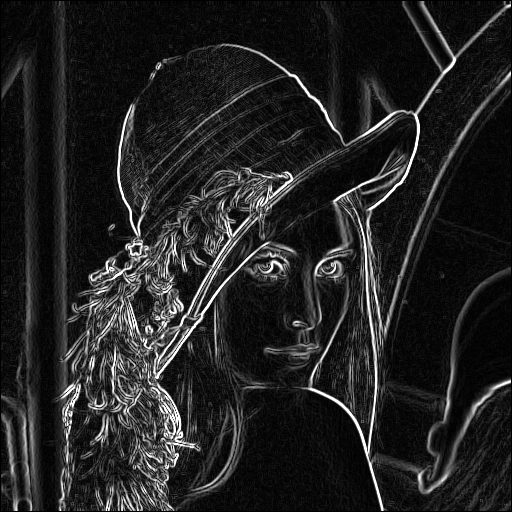
\includegraphics[scale=0.25]{Image/filtrePrewittBidirectionnel.png}
			\caption{Prewitt Bidirectionnel}
			\label{fig:PrewittBidirectionnel}
		\end{minipage} \hfill
		\begin{minipage}[c]{.3\linewidth}
		\centering
			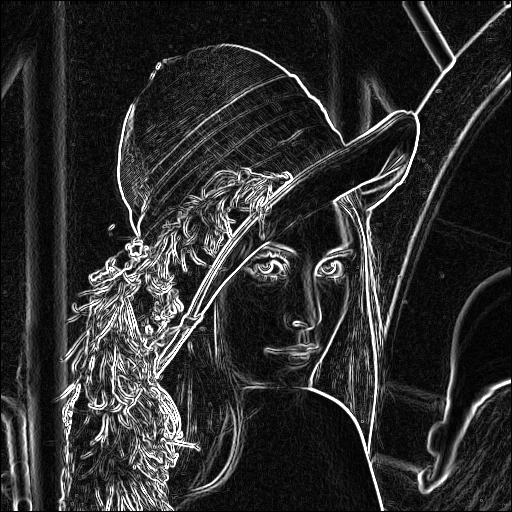
\includegraphics[scale=0.25]{Image/filtreSobelBidirectionnel.png}
			\caption{Sobel Bidirectionnel}
			\label{fig:SobelBidirectionnel}
		\end{minipage}\hfill
		\begin{minipage}[c]{.3\linewidth}
		\centering
		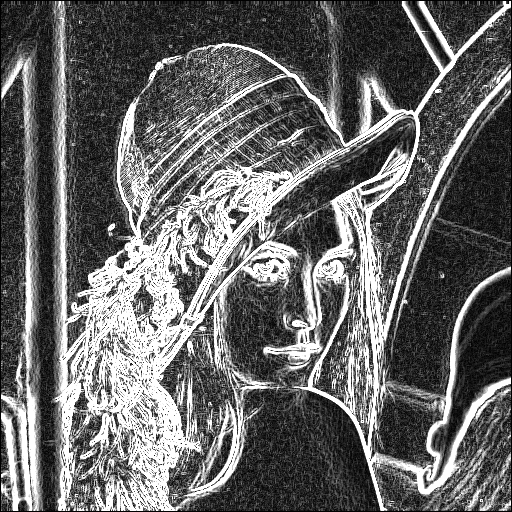
\includegraphics[scale=0.25]{Image/filtreKirschBidirectionnel.png}
		\caption{Kirsch Bidirectionnel}
		\label{fig:KirschBidirectionnel}
		\end{minipage}
	\end{figure}

	L’avantage de cette méthode est que seul 2 filtres sont nécessaires pour calculer le gradient en 1 point. 
	Cependant elle peut être plus sensible au bruit que la méthode multidirectionelle.

	Après le calcul des gradients horizontaux et verticaux, on peut calculer l'orientation du gradient.
	Pour celà, on utilise la formule :
	$$
		\theta = \arctan(\frac{G_{h}}{G_{v}})
	$$

	Pour calculer cette orientation, nous avons utiliser la fonction atan2(x,y)	qui en C++ calcule $\arctan(\frac{x}{y})$. 
	Le resultat de cette fonction est compris entre $-\pi$ et $\pi$.

	Une fois cette orientation calculée, mous pouvons affiché les différents angles récupés dans différentes couleurs :
	\begin{itemize}
	\item Entre 0 et $\pi/2$, rouge.
	\item Entre $\pi/2$ et $\pi$, vert.
	\item Entre 0 et $-\pi/2$, bleu.
	\item Entre $-\pi/2$ et $-\pi$, blanc.
	\end{itemize}
            
	\begin{figure}[H]
		\begin{minipage}[c]{.3\linewidth}
			\centering
			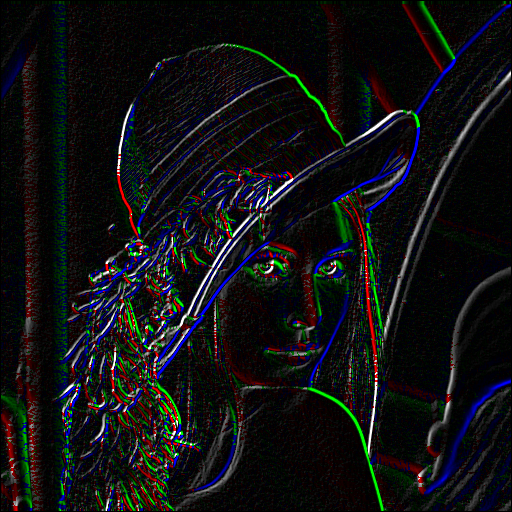
\includegraphics[scale=0.25]{Image/filtrePrewittBidirectionnelCouleur.png}
			\caption{Prewitt Bidirectionnel Couleur}
			\label{fig:PrewittBidirectionnelCouleur }
		\end{minipage} \hfill
		\begin{minipage}[c]{.3\linewidth}
		\centering
			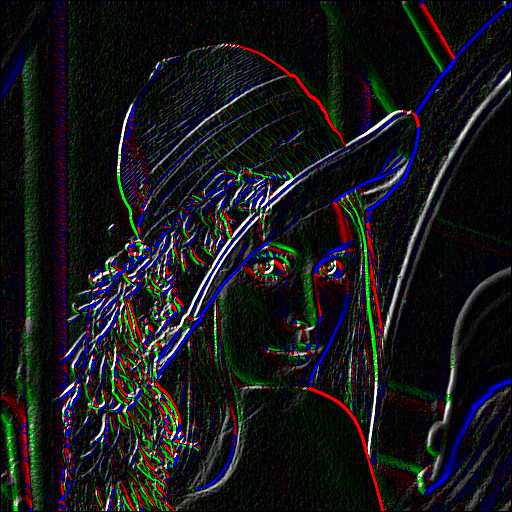
\includegraphics[scale=0.25]{Image/filtreSobelBidirectionnelCouleur.png}
			\caption{Sobel Bidirectionnel Couleur}
			\label{fig:SobelBidirectionnelCouleur}
		\end{minipage}\hfill
		\begin{minipage}[c]{.3\linewidth}
		\centering
		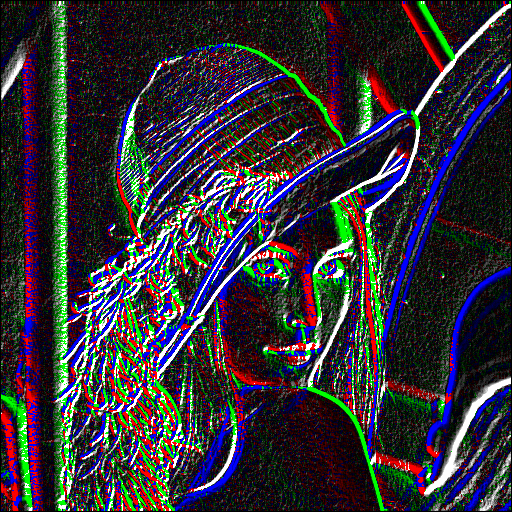
\includegraphics[scale=0.25]{Image/filtreKirschBidirectionnelCouleur.png}
		\caption{Kirsch Bidirectionnel Couleur}
		\label{fig:KirschBidirectionnelCouleur}
		\end{minipage}
	\end{figure}


	Comme les deux filtres sont calculés sur la même de l'image, la complexité est également de \[w \times h\].

	\subsection{Filtrage multidirectionnel}

	Pour le calcul du filtre multidirectionnel deux masques diagonaux sont rajoutés, voici ceux du filtre de Prewitt:
	\\
	\begin{tabular}{cccc}
		Diagonal gauche &
		$
		\begin{pmatrix}
			1 & 1 & 0 \\
			1 & 0 & -1 \\
			0 & -1 & -1
		\end{pmatrix}
		$
		& Diagonal droite &
		$
		\begin{pmatrix}
		0 & 1 & 1 \\
		-1 & 0 & 1 \\
		-1 & -1 & 0
		\end{pmatrix}
		$
	\end{tabular}

	Ces filtres donnent : 

	\begin{figure}[H]
		\begin{minipage}[c]{.46\linewidth}
			\centering
			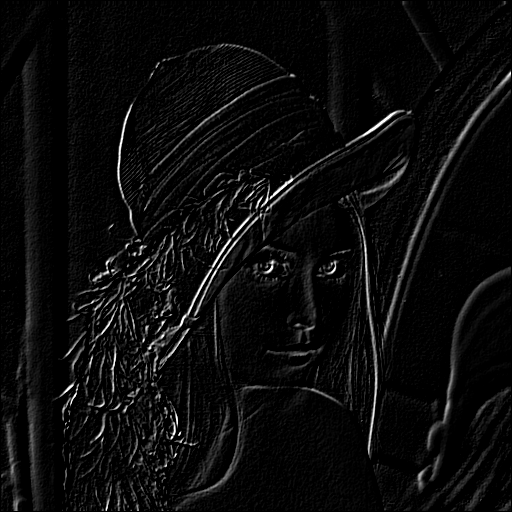
\includegraphics[scale=0.25]{Image/filtrePrewittDiagonalG.png}
			\caption{Prewitt Diagonal Gauche}
			\label{fig:PrewittDiagonalG}
		\end{minipage} \hfill
		\begin{minipage}[c]{.46\linewidth}
		\centering
			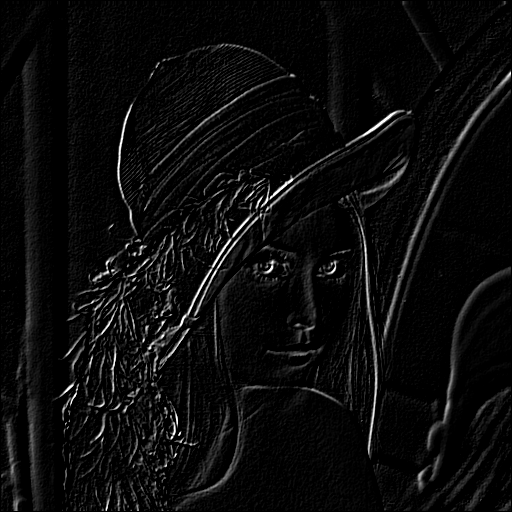
\includegraphics[scale=0.25]{Image/filtrePrewittDiagonalD.png}
			\caption{Prewitt Diagonal Droite}
			\label{fig:SobelDiagonalD}
		\end{minipage}
	\end{figure}

	Le filtre multidirectionnel calcule donc un filtre bidirectionnel avec les filtres diagonaux correspondants.

	\begin{figure}[H]
		\begin{minipage}[c]{.46\linewidth}
			\centering
			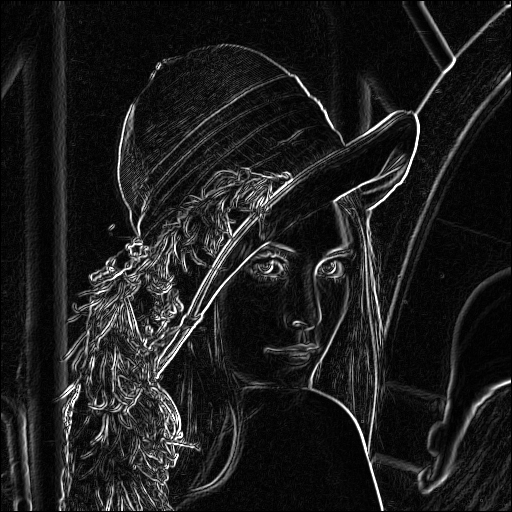
\includegraphics[scale=0.25]{Image/filtrePrewittMultidirectionnel.png}
			\caption{Prewitt Multidirectionnel}
			\label{fig:PrewittMultidirectionnel}
		\end{minipage} \hfill
		\begin{minipage}[c]{.46\linewidth}
		\centering
			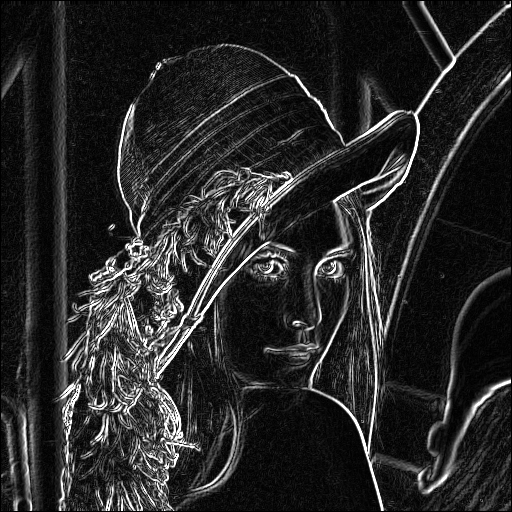
\includegraphics[scale=0.25]{Image/filtreSobelMultidirectionnel.png}
			\caption{Sobel Multidirectionnel}
			\label{fig:SobelMultidirectionnel}
		\end{minipage}
	\end{figure}

	\begin{figure}[H]
		\centering
		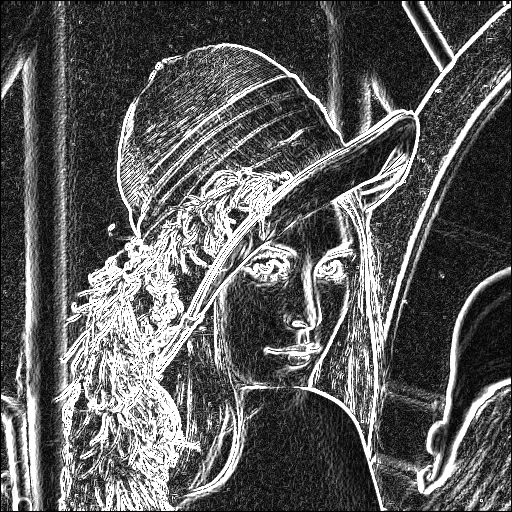
\includegraphics[scale=0.25]{Image/filtreKirschMultidirectionnel.png}
		\caption{Kirsch Multidirectionnel}
		\label{fig:KirschMultidirectionnel}
	\end{figure}

	Pour calculer l'orientation du filtre, on récupère la maximum des gradients calculés pour le points.

	Le choix de la couleur en fonction du maximum choisi.

	\begin{itemize}
	\item masque Vertical, rouge.
	\item masque Horizontal, vert.
	\item masque Diagonal droite, bleu.
	\item masque Diagonal gauche, blanc.
	\end{itemize}
            
	\begin{figure}[H]
		\begin{minipage}[c]{.3\linewidth}
			\centering
			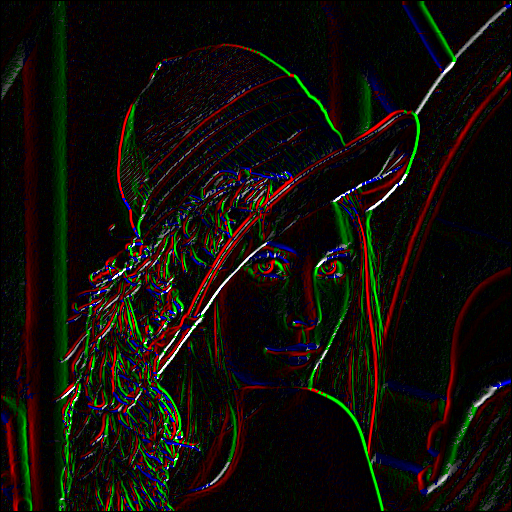
\includegraphics[scale=0.25]{Image/filtreMultidirectionnelPrewittCouleur.png}
			\caption{Prewitt Multidirectionnel Couleur}
			\label{fig:PrewittMultidirectionnelCouleur }
		\end{minipage} \hfill
		\begin{minipage}[c]{.3\linewidth}
		\centering
			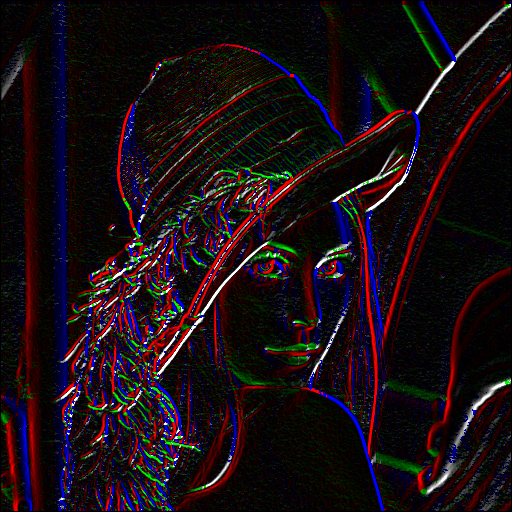
\includegraphics[scale=0.25]{Image/filtreMultidirectionnelSobelCouleur.png}
			\caption{Sobel Multidirectionnel Couleur}
			\label{fig:SobelMultidirectionnelCouleur}
		\end{minipage}\hfill
		\begin{minipage}[c]{.3\linewidth}
		\centering
		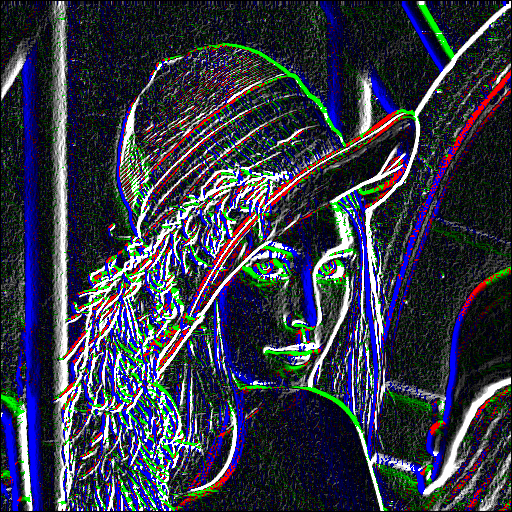
\includegraphics[scale=0.25]{Image/filtreMultidirectionnelKirschCouleur.png}
		\caption{Kirsch Multidirectionnel Couleur}
		\label{fig:KirschMultidirectionnelCouleur}
		\end{minipage}
	\end{figure}

	Le calcul des masques se faisant toujours en un seul passage sur l'image, la complexité ne change pas.

	L'utilisation de plus de filtre permet de réduire le bruit sur la detection des contours. 
	Néanmoins, ce bruit est toujours présent, c'est pourquoi il faut passer à l'étape du seuillage.
 
\section{Seuillage}
	
	Le seuillage consiste à "filtrer" les pixels de l'image filtrer en fonction d'un seuil. 
	Si la valeur du pixel courant est inférieur au seuil, elle est passée à 0, sinon elle prend la valeur maximale (ici 255).

	Celui ci peut être déterminer de plusieurs manière.

	\subsection{Implémentation}

	Pour le seuillage, il n' y a qu'une seule classe seuillage qui contient l'image filtrée et l'image seuillé avec que celle ci soit affinée.

	Les différentes fonctions de seuillage retournent une image et ne prennent aucun arguments (sauf seuilFixe() et SeuilHysteresis() qui prennent les valeurs des seuils comme expliqué ci dessous. (voir \ref{fixe} et \ref{hysteresis}) ).

	\subsection{Seuillage fixe}\label{fixe}

	Le seuil S est fixé et est commun à toute l'image. néanmoins il faut choisir une bonne valeur pour avoir un résultat correct.

	Les exemples ci-dessous ont été calculé sur un filtre de Prewitt multidirectionnel.
	\begin{figure}[H]
		\begin{minipage}[c]{.30\linewidth}
			\centering
			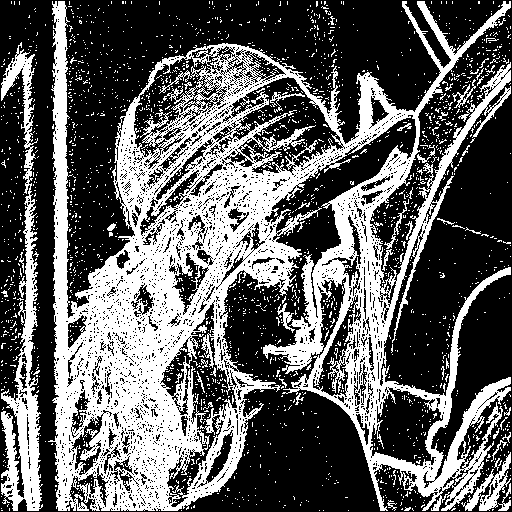
\includegraphics[scale=0.15]{Image/seuilFixe20.png}
			\caption{S = 20}
			\label{fig:seuilFixe20}
		\end{minipage} \hfill
		\begin{minipage}[c]{.30\linewidth}
			\centering
			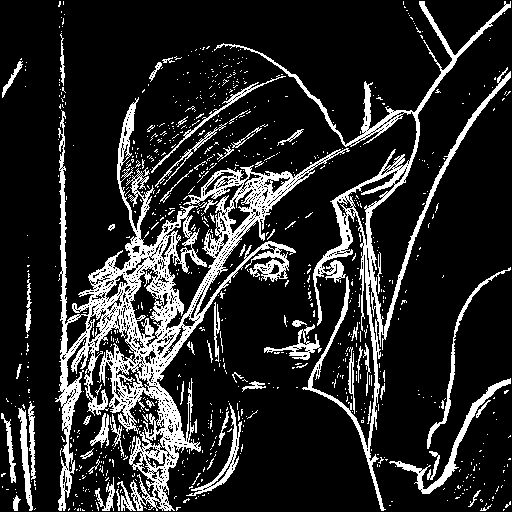
\includegraphics[scale=0.15]{Image/seuilFixe50.png}
			\caption{S = 50}
			\label{fig:seuilFixe50}
		\end{minipage} \hfill
		\begin{minipage}[c]{.30\linewidth}
			\centering
			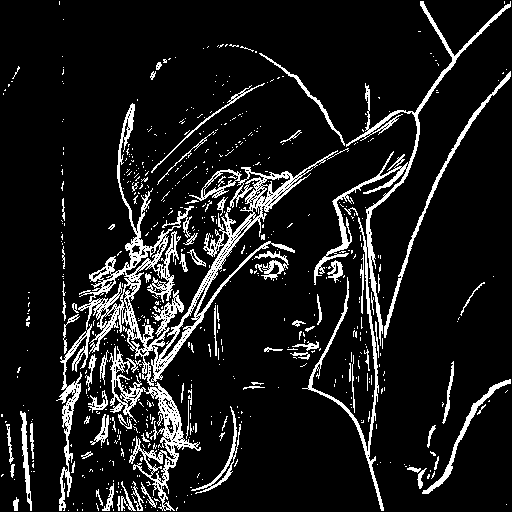
\includegraphics[scale=0.15]{Image/seuilFixe70.png}
			\caption{S = 70}
			\label{fig:seuilFixe70}
		\end{minipage}

		\begin{minipage}[c]{.30\linewidth}
			\centering
			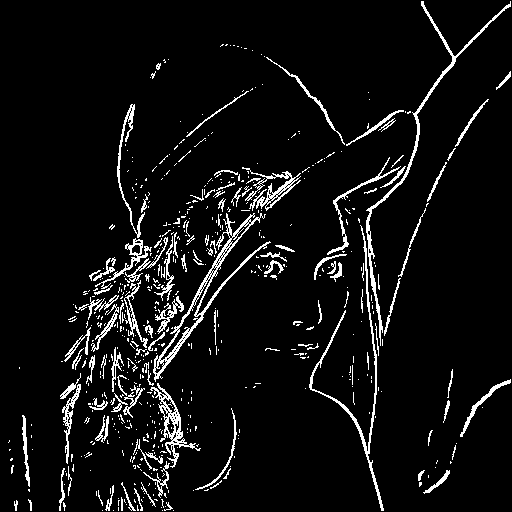
\includegraphics[scale=0.15]{Image/seuilFixe100.png}
			\caption{S = 100}
			\label{fig:SeuilFixe100}
		\end{minipage} \hfill
		\begin{minipage}[c]{.30\linewidth}
			\centering
			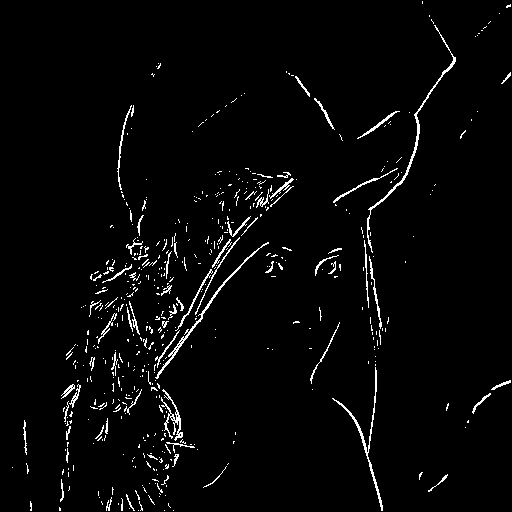
\includegraphics[scale=0.15]{Image/seuilFixe150.png}
			\caption{S = 150}
			\label{fig:seuilFixe150}
		\end{minipage} \hfill
		\begin{minipage}[c]{.30\linewidth}
			\centering
			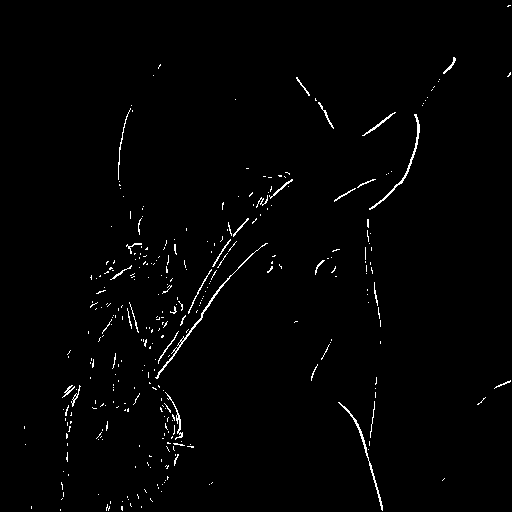
\includegraphics[scale=0.15]{Image/seuilFixe200.png}
			\caption{S = 200}
			\label{fig:seuilFixe200}
		\end{minipage}
	\end{figure}

	Pour des seuils très bas, on  remarque bien que le bruit est important (figure \ref{fig:seuilFixe20}).
	Au contraire, dans le cas de seuil élevé, certain contours sont effacés et l'image perd en précision (figure \ref{fig:seuilFixe150} et \ref{fig:seuilFixe200}).

	La compléxité de cette méthode est de \[w \times h\]

	\subsection{Seuillage global}

	Nous venons de voir que le choix du seuil est crucial dans le seuillage de l'image. 
	Il est rapidement contraignant de chercher "à la main" le seuil optimal pour une image.
	Le seuillage globale permet de determiner un seuil pour une image : il calcule la valeur moyenne des gradients de l'image et 
	prend cette moyenne comme seuil.

	\begin{figure}[H]
		\centering
		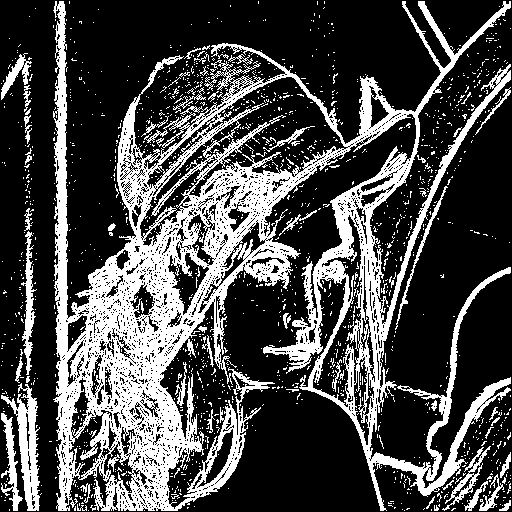
\includegraphics[scale=0.25]{Image/seuilGlobal.png}
		\caption{Seuillage Global de Prewitt multidirectionnel}
		\label{fig:seuilGlobal}
	\end{figure} 

	La complexité est plus grande car on effectue deux parcours de l’image: \[2 \times w \times x\]

	L’image contenant beaucoup de nuances de gris comme contours, le résultat contient beaucoup de "bruit" dans les contours.

	\subsection{Seuillage local}

	Le seuillage local calcule la moyenne des pixels voisins au pixel courant. 
	Une fois cette moyenne calculé, on la compare avec le pixel courant.

	\begin{figure}[H]
		\centering
		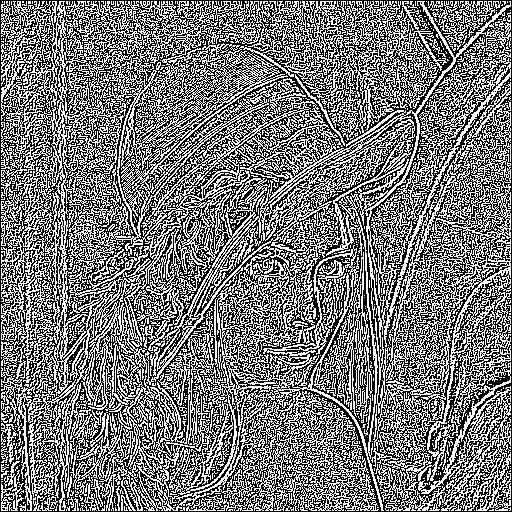
\includegraphics[scale=0.25]{Image/seuilLocal.png}
		\caption{Seuillage Local de Prewitt multidirectionnel}
		\label{fig:seuilLocal}
	\end{figure} 

	Le résultat est  bruité mais celui-ci a une précision supérieur à celle du seuil global. 
	En effet, on retrouve toute les courbes intacts dans l'image seuillée.

	La complexité est plus élevée a cause du calcul systématique de la moyenne locale: \[l^2 \times w \times x\]
	avec \textit{l} la taille de la zone où est calculé la moyenne.

	\subsection{Seuillage par Hysteresis}\label{hysteresis}

	Dans le cas d'un seuillage par hysteresis, on utilise deux seuil, un seuil Bas \textit{Sb} et un seuil haut \textit{Sh}.

	\begin{verbatim}
		Si Pixel_courant < Sb alors Pixel_courant = 0
		Sinon Si Pixel_courant > Sh alors Pixel_courant = 255
		Sinon Si un voisin de Pixel_courant = 225 alors Pixel_courant = 255
		      Sinon Pixel_courant = 255
	\end{verbatim}

	\begin{figure}[H]
		\centering
		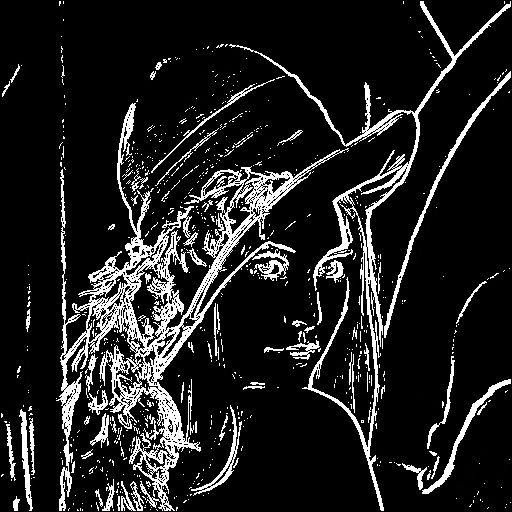
\includegraphics[scale=0.25]{Image/seuilHysteresis.png}
		\caption{Seuillage Hysteresis de Prewitt multidirectionnel	(\textit{Sb} = 44, \textit{Sh} = 60)}
		\label{fig:seuilHysteresis}
	\end{figure} 



	Cet algorithme permet de réduire le bruit et les trous dans les contours et donne d'excellents résultats.

	La difficulté de cette méthode est dans le choix des valeurs de \textit{Sb} et \textit{Sh}.
	Les mêmes problèmes que le seuillage fixe peuvent se produire. (voir \ref{fixe}).

	La complexité de cette algorithme est de \[n \times w \times h\]
	avec \textit{n} le nombre de passage sur l'image pour controler les pixel entre deux valeurs.

	Une fois, les contours bien définis par le seuillage, il reste encore une étape : l'affinage.


\section{Affinage}

	\subsection{Algorithme}
		La détection de contours a pour conséquences de générer, pour chaque contours de l'image, des points doubles : l'un correspond à la frontière d'une zone, et l'autre à la frontière de la zone voisine. 
		L'affinage des contours consiste obtenir de un pixel d'épaisseur. 
		Pour y parvenir, la méthode d'extraction des maximas locaux dans la direction du gradient a été utilisée.

		Le pixel (\textit{m},\textit{n}) est un contour horizontal si : \\
		$$
			|G_{v}| > |G_{h}| 
		$$	
		$$
			G(m,n) > S 
		$$	
		$$
			G(m,n) \le G(m - 1, n)\ et\ G(m, n) > G(m + 1, n) 
	    $$

	    avec : 
	    \begin{itemize}
		    \item $G_{v}$ le gradient vertical,
		    \item $G_{h}$ le gradient horizontal,
		    \item $G$ le module du gradient,
		    \item $S$ le seuil.

	    \end{itemize}

	    Le pixel (\textit{m},\textit{n}) est un contour vertical si : \\
		$$
			|G_{h}| > |G_{v}| 
		$$	
		$$
			G(m,n) > S 
		$$	
		$$
			G(m,n) \ge G(m, n - 1)\ et\ G(m, n) > G(m , n + 1) 
	    $$


	    Si un point n'est pas un maximum local, il peut être supprimé. 
	    C’est grâce à cette méthode que nous éliminons entre autre les points doubles générés par l’étape de détection. 
	    La complexité de l’algorithme d’affinage revient toujours à l’ordre d’un parcours de l’image.

    \subsection{Implémentation}

    	La fonction d'affinage utilise une fonction déjà filtrée et seuillé.
    	Elle récupère également les tableaux des gradients horizontaux et verticaux.
    	Avec Celà, on applique l'algorithme décrit ci-dessus.
    	Le points est affiché dans l'image affiné uniquement s'il est un maximum local.

    \subsection{Exemple}

		\begin{figure}[H]
			\centering
			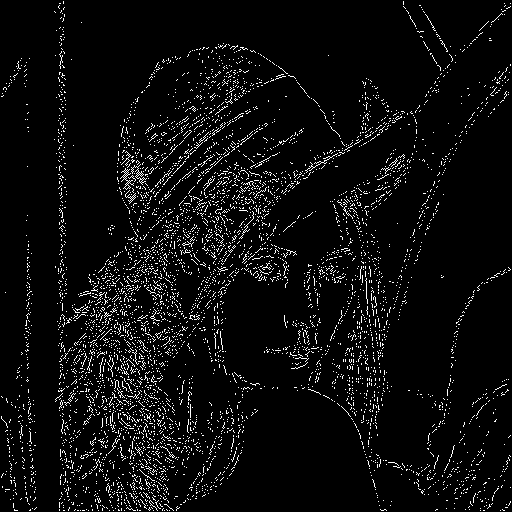
\includegraphics[scale=0.25]{Image/affinage.png}
			\caption{affinage du seuillage Hysteresis (figure \ref{fig:seuilHysteresis})}
			\label{fig:affinage}
		\end{figure} 

\section{Conclusion}

	Nous avons réussi à détecter les contours dans une image en utilisant différents masques de convolution. 
	Quelques imperfections subsistent, mais ces opérateurs nous ont déjà démontré leur efficacité. 

	Pendant ce TP, nous avons implémenté beaucoup d’algorithmes qui ont une complexité de l’ordre de la taille de l’image. 


\end{document}

%\begin{figure}[H]
%      \centering
 %     \includegraphics[scale=0.7]{Image/grandTableau.png} 
 %     \caption{Position de départ}
%      \label{fig:grandTableau}
%  \end{figure}

%	\[
%	\begin{pmatrix}
%	1 & 2 & 3 \\
%	4 & 5 & 6 \\
%	7 & 8 & 9
%	\end{pmatrix}
%	\]
